\documentclass[10pt,a4paper]{book}
\usepackage[utf8]{inputenc}
\usepackage[spanish]{babel}
\usepackage{amsmath}
\usepackage{amsfonts}
\usepackage{amssymb}
\usepackage{makeidx}
\usepackage{graphicx}
\usepackage{listings}
\lstset{language=bash,breaklines=true}
\author{José Jácome,Erik Quijije}
\title{Tutorial Máxima}
\usepackage{listings}
\usepackage{color}
\usepackage{inputenc}
%\lstset{language=Lisp}
\begin{document}
\begin{titlepage}
 \begin{center}
  \vspace*{-1in}
  \begin{figure}[htb]
   \begin{center}
    
\includegraphics[width=8cm]{espe.jpg}
   \end{center}
 \end{figure}

  INGENIERIA MECATRÓNICA\\
  \vspace*{0.15in}
  DEPARTAMENTO DE CIENCIAS EXACTAS\\
  \vspace*{0.6in}
  \begin{Large}
   \textbf{LIBRO DE MATEMATICAS SUPERIOR} \\
   \author{Maqueavelo Hidrovo}
   \author{José Jácome}
   \author{Erik Quijije}
  \end{Large}
  \vspace*{0.3in}
  \begin{large}
   Supervisado por: \\
   Dr. Marcelo Roman \\
   2014\\
  \end{large}
 \end{center}
\end{titlepage}

\chapter{Primeros pasos con WXMaxima}
\section{Que es Máxima?}
\begin{small}
El sistema de álgebra computacional Maxima es un motor de cálculo simbólico escrito en lenguaje Lisp publicado bajo licencia GNU GPL.\\
Cuenta con un amplio conjunto de funciones para hacer manipulación simbólica de polinomios, matrices, funciones racionales, integración, derivación, manejo de gráficos en 2D y 3D, manejo de números de coma flotante muy grandes, expansión en series de potencias y de Fourier, entre otras funcionalidades.\\
Maxima funciona en modo consola, sin embargo incluye las intefaces gráficas xMaxima y wxMaxima para facilitar su uso.\\
\section{Instalacion de WXMaxima en GNU-Linux}
\subsection{Debian, Ubuntu y Derivadas}
Para instalar máxima en una distribución Debian Ubuntu y derivados es tan dificil como hacer:\\
\begin{enumerate}

\begin{figure}[htb]
\item Instalamos maxima:\\
\begin{center}
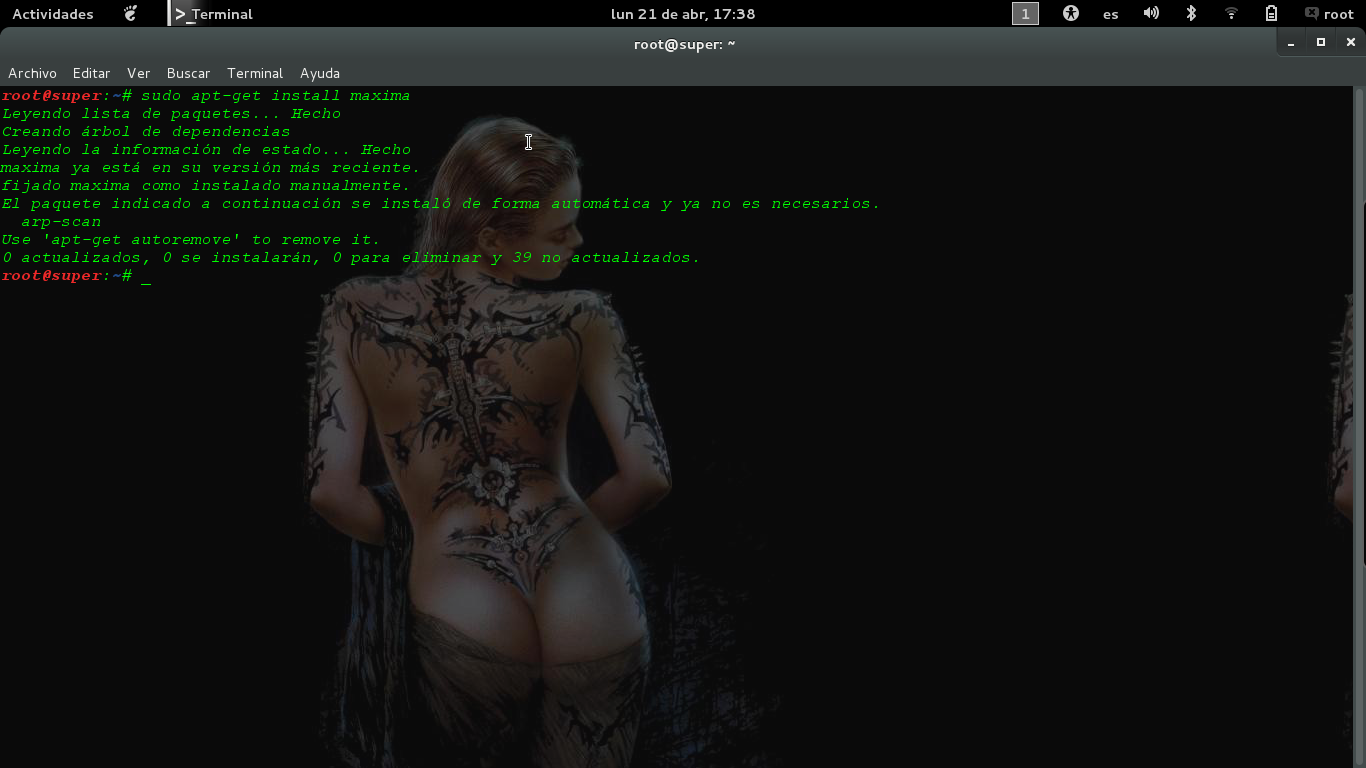
\includegraphics[width=13cm]{fotos/cap2}
\begin{lstlisting}
	sudo apt-get install maxima
\end{lstlisting}
%\caption{\textbf{}}
\end{center}
\end{figure}


\begin{figure}[htb]
\item Instalamos las librerías necesarias para que funcione wxmaxima:\\
\begin{center}
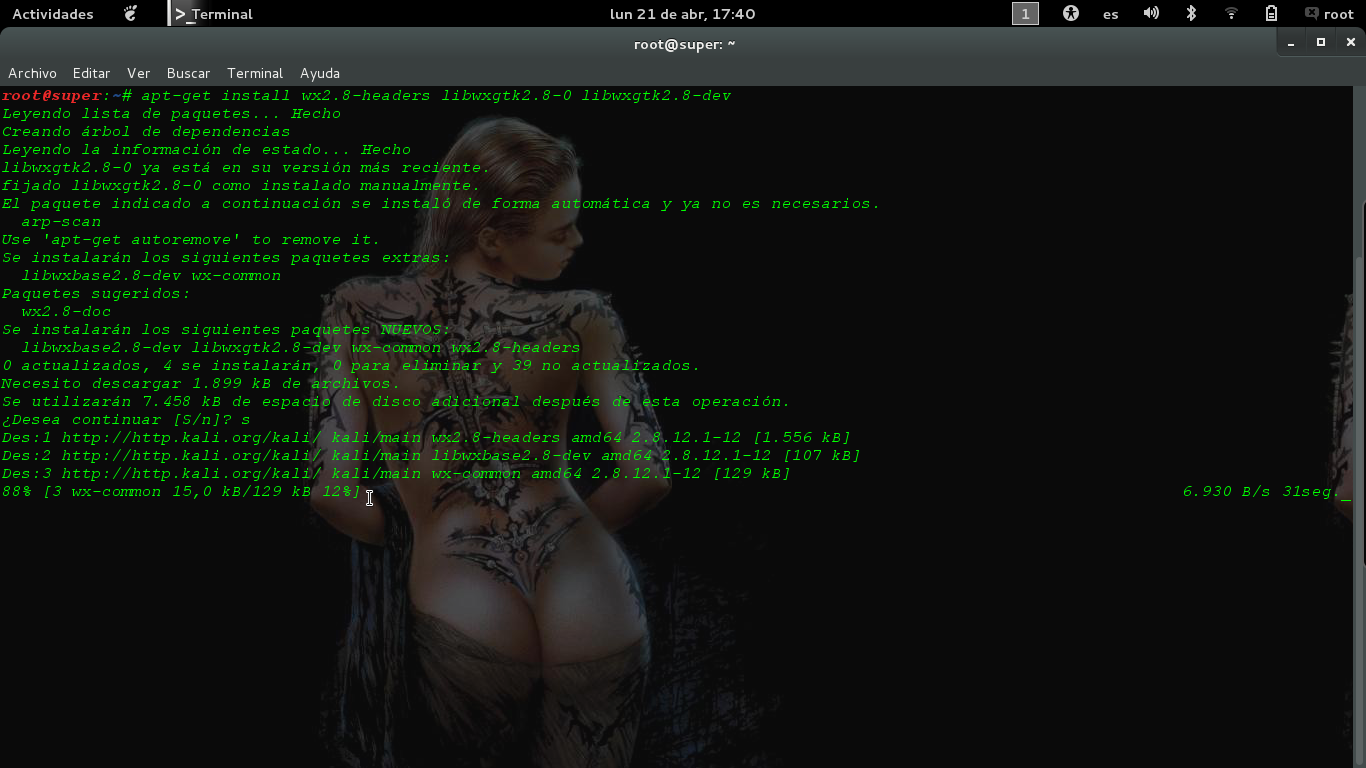
\includegraphics[width=13cm]{fotos/cap4}
\caption{\textbf{sudo apt-get install wx2.8-headers libwxgtk2.8-0 libwxgtk2.8-dev}}
\end{center}
\end{figure}


\begin{figure}[htb]
\item Instalamos wxmaxima:\\
\begin{center}
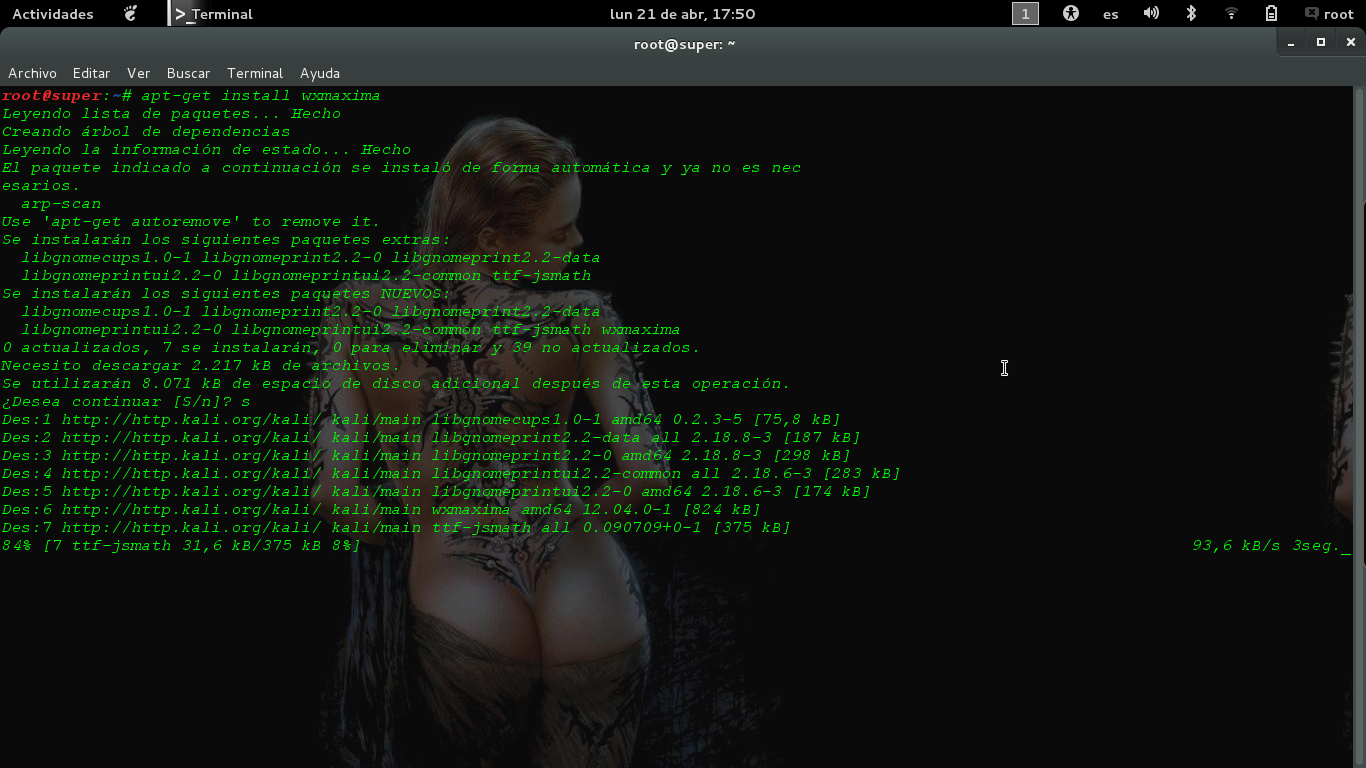
\includegraphics[width=13cm]{fotos/cap6}
\caption{\textbf{sudo apt-get install wxmaxima}}
\end{center}
\end{figure}


\begin{figure}[htb]
Si todo ha ido bien, debería ser posible ejecutar el editor WxMaxima:\\
\begin{center}
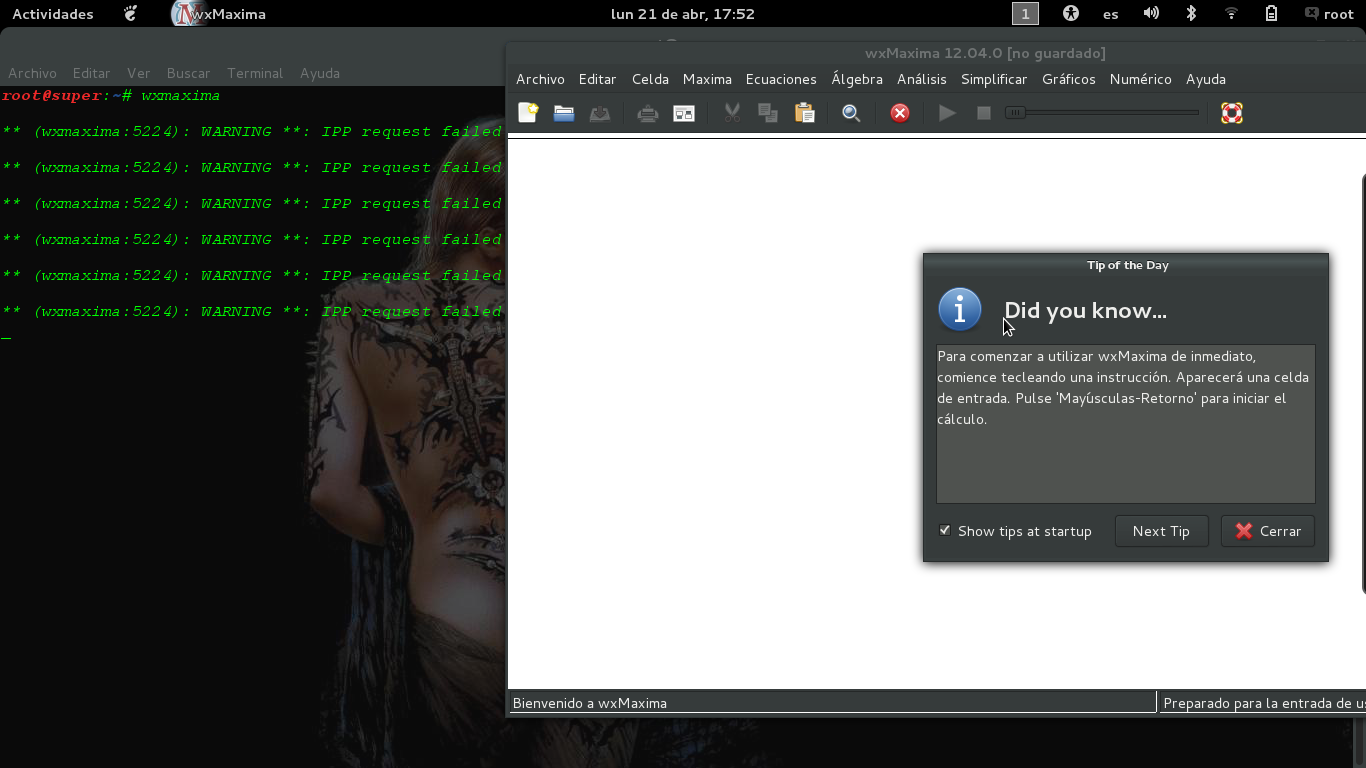
\includegraphics[width=13cm]{fotos/cap7}
\caption{\textbf{Corriendo la interfaz}}
\end{center}
\end{figure}
\end{enumerate}
\begin{figure}[htb]
\subsection{Arch Linux y Derivadas (Manjaro, Antergos, Chakra)}
Para poder instalar WxMaxima eng Arch Linux utilizamos el siguiente comando en un terminal:
\begin{center}
	\begin{lstlisting}
	sudo pacman -S wxmaxima maxima
\end{lstlisting}
\end{center}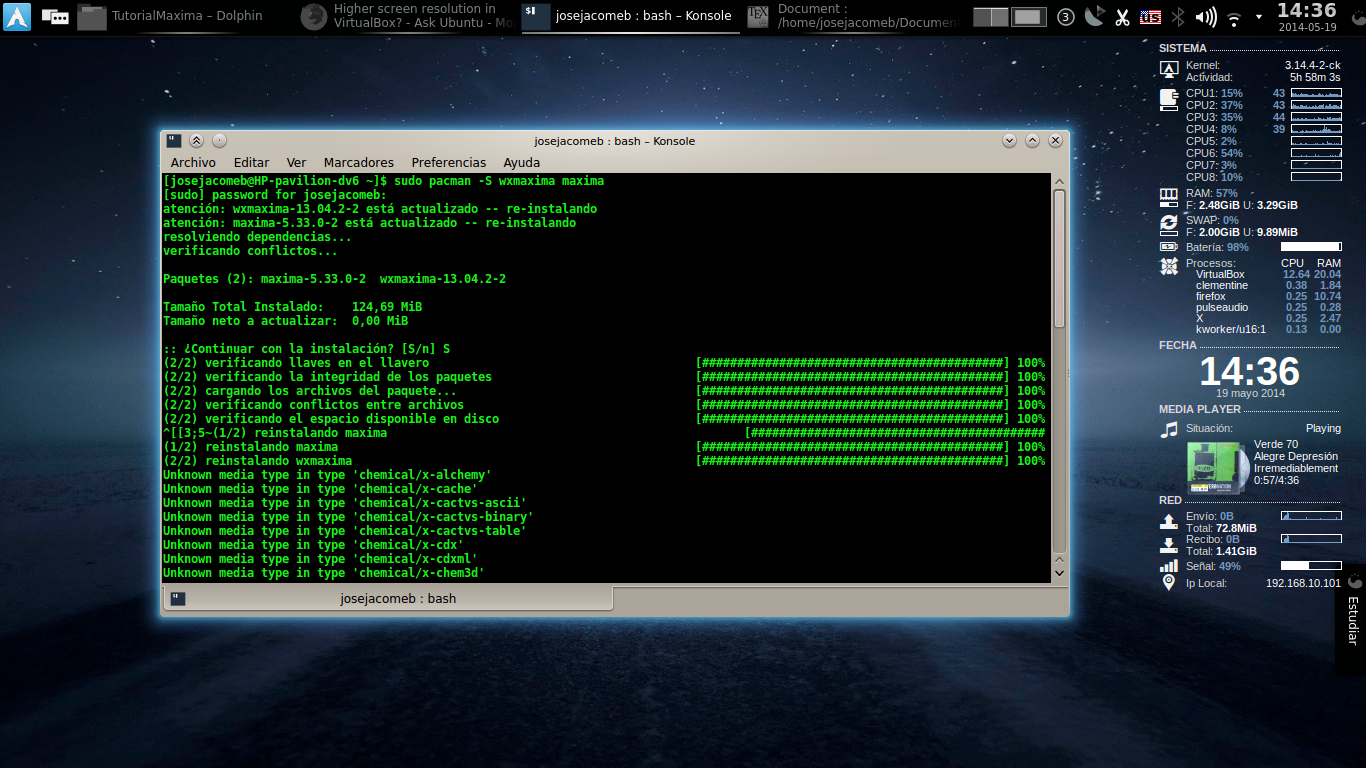
\includegraphics[scale=0.30]{fotos/Maxima.png} \\
Después de estos buscamos en nuestro menú de aplicaciones\\ 
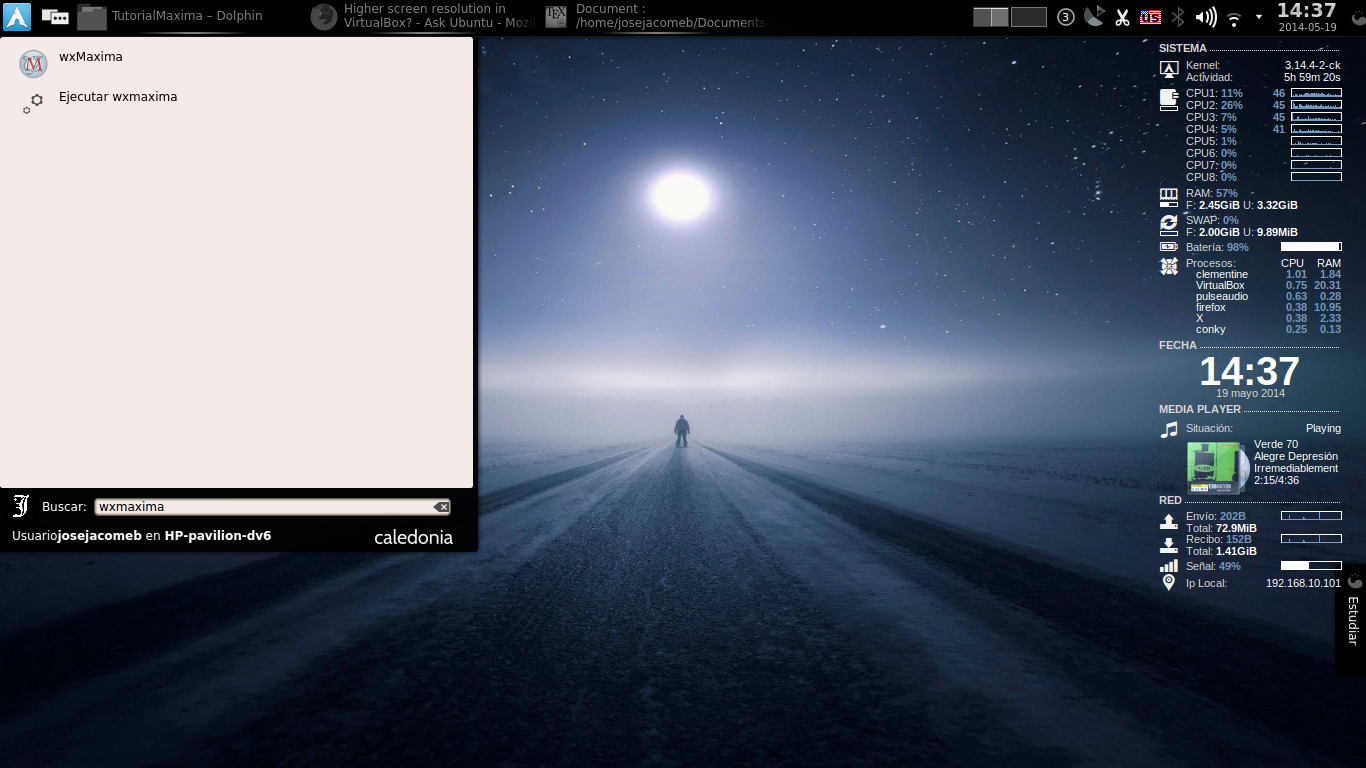
\includegraphics[scale=0.30]{fotos/Maxima1.png} \\
Si logramos encontrarlo, ejecutamos el programa tal como nos muestra la Captura\\ 
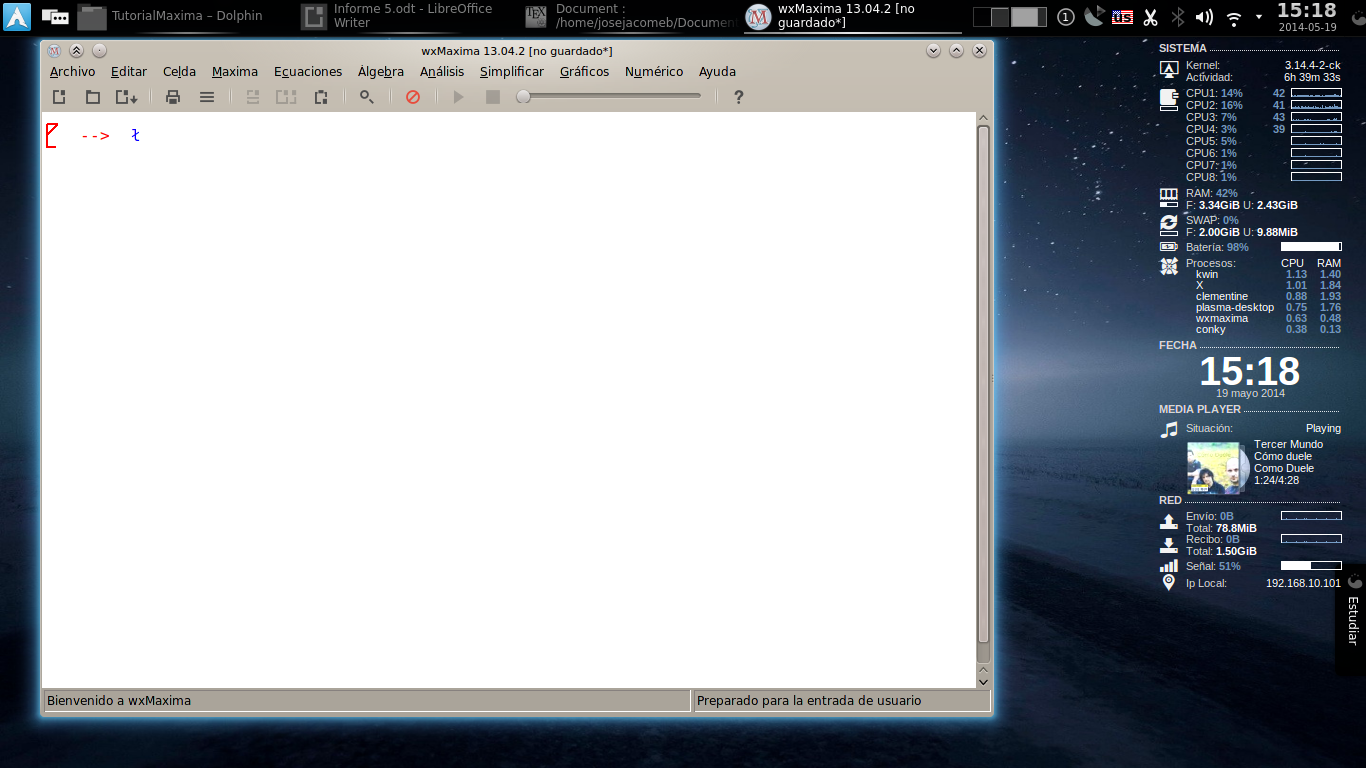
\includegraphics[scale=0.35]{fotos/Maxima2.png} \\
\section{Interfaz de MXMaxima}

Maxima es un programa que se ha diseñado para funcionar en una terminal de texto y aqui veremos el uso de Maxima con la interface de texto donde ejecutamos la terminal y escribimos maxima.\\

Utilizamos una sencilla ecuacion para obtener sus raices y observar el funcionamiento donde el resultado se entiende pero no es demasiado legible:\\
\begin{center}
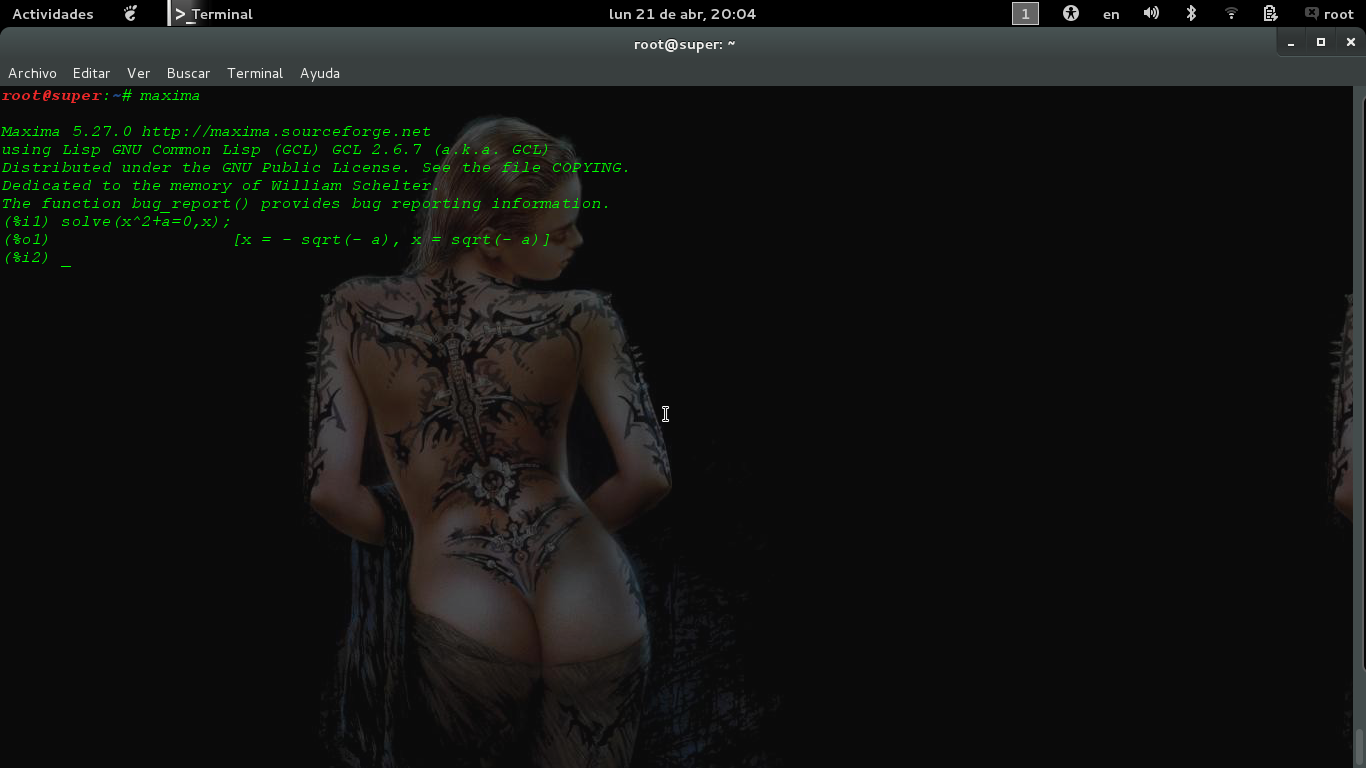
\includegraphics[width=13cm]{fotos/cap8}
\caption{\textbf{Interfaz de texto y las raices de la ecuacion $x^2+a=0$}}


\end{center}
Lastimosamente ya no es un entorno de trabajo aceptable, En cambio al realizar la misma operacion en WXMaxima la resolucion suele ser mucho mas intuitivo.
\end{figure}

\begin{figure}[htb]
\begin{center}
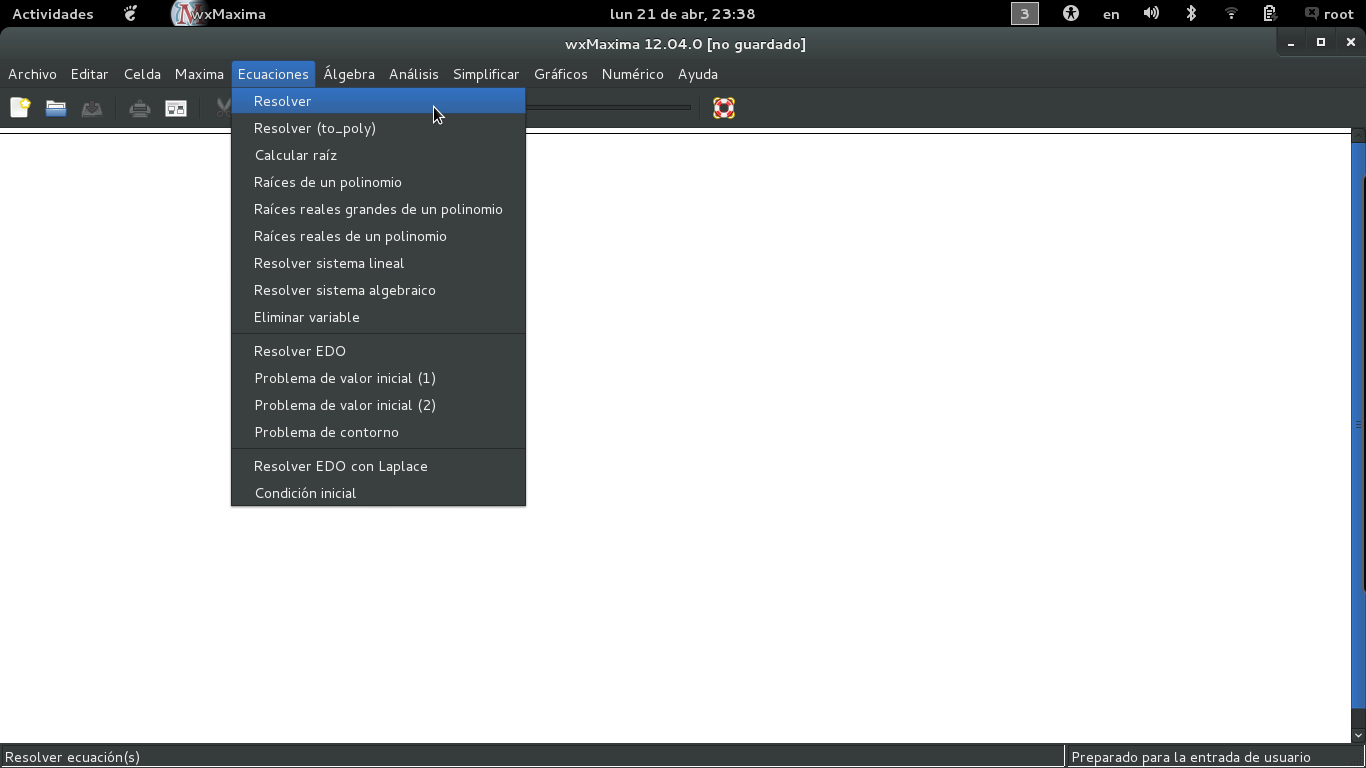
\includegraphics[width=13cm]{fotos/cap9.png}
\caption{\textbf{Entorno amigable}}
\end{center}
\end{figure}

\begin{figure}[htb]
En si WXMaxima tiene algunas opciones disponibles y faciles de utilizar y muchos botones o iconos de acceso rapido como ejemplo abrir, guardar sesion, imprimir, cambiar propiedades de WXMaxima, interrumpir calculo actual, contro de graficos animados y un acceso directo a la ayuda del programa.
Otra area a mostrar es la de trabajo donde se le dice a WXMaxima que es lo que quiero realizar y donde se muestra los resultados.
\begin{center}
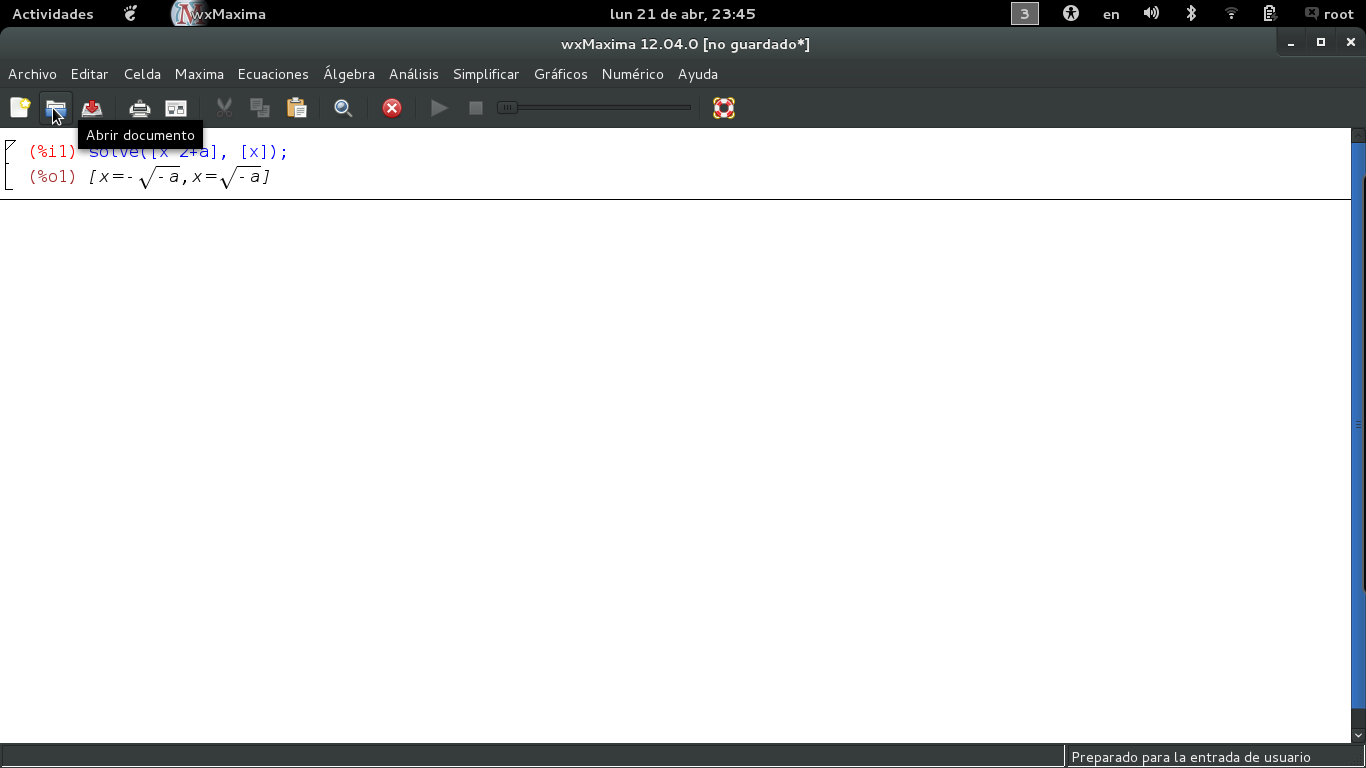
\includegraphics[width=13cm]{fotos/cap10.png}
\caption{\textbf{ }}
\end{center}
\end{figure}

\begin{figure}[htb]
Uno de los elementos mas importantes de WXMaxima es la ayuda la cual tiene el manual de referencia en el idioma de ingles.\\
Podemos buscar referencias a partir del Indice o Buscar, digitamos como es en este caso Laplace y nos muestra manuales o capitulos respectivamente donde aparezca las coincidencias de busqueda.
\begin{center}
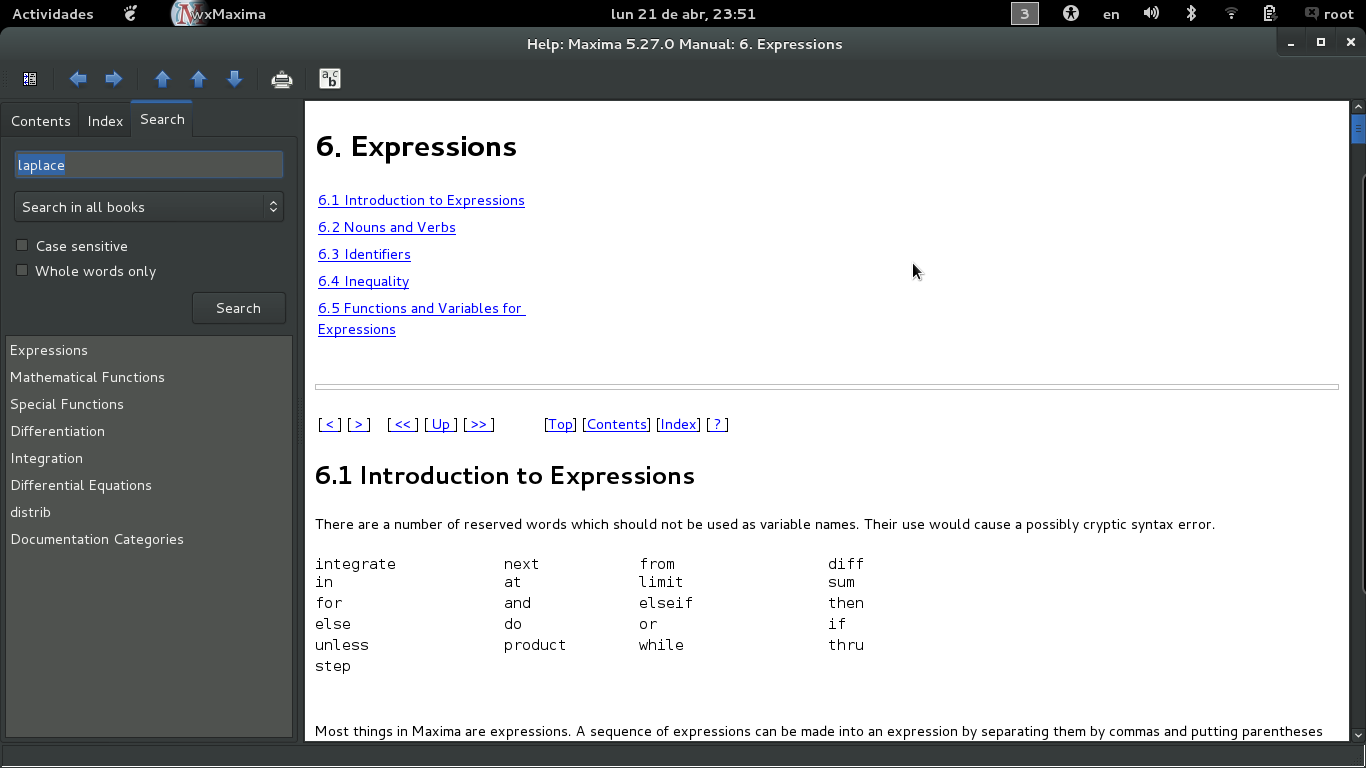
\includegraphics[width=13cm]{fotos/cap11}
\caption{\textbf{Manual de ayuda}}
\end{center}
\end{figure}

\begin{figure}[htb]
%\vspace*{-2,5in}
En el menu de ayuda se nos muestra varias pestañas de mucha utilidad principalmente el de ejemplo que tiene como objetivo orientarnos con algun tipo de ejercicio resuelto.
\begin{center}

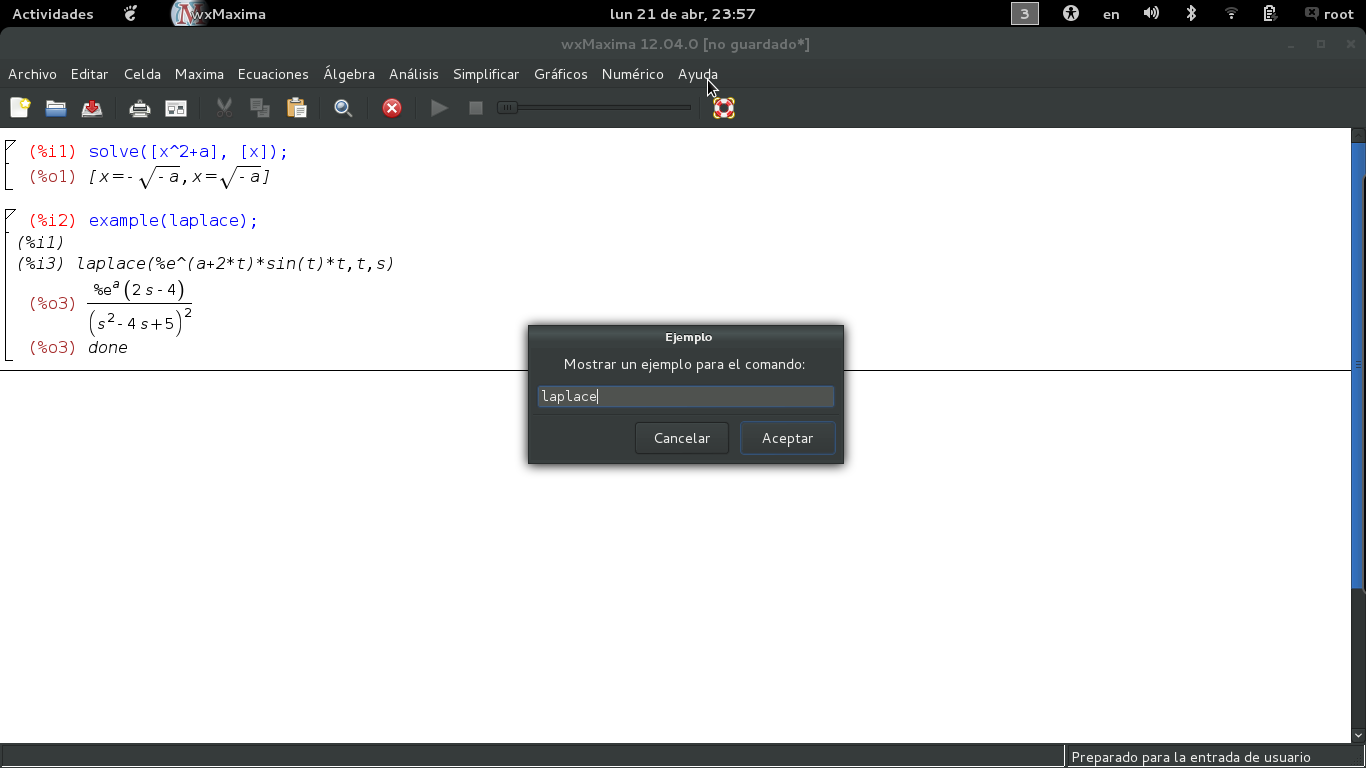
\includegraphics[width=13cm]{fotos/cap12}
\caption{\textbf{Ejemplos}}
\end{center}
\end{figure}
\end{small}
\chapter{Graficas con WXMaxima}
\section{Tipos de comandos}
\begin{small}

\begin{itemize}
\item $gnuplot$ (formato por defecto para Windows)

Se utiliza para ejecutar el programa externo Gnuplot, el cual debe estar instalado en el sistema. Las instrucciones gráficas y los datos se almacenan en el fichero maxout.gnuplot.

\item $gnuplot_pipes$ (formato por defecto para plataformas distintas de Windows)

Este formato no está disponible en plataformas Windows. Es similar al formato gnuplot, excepto por el hecho de que las instrucciones son enviadas a $Gnuplot$ por una tubería, mientras que los datos se almacenan en el fichero $maxout.gnuplot_pipes$. 
Mediante esta técnica, un único proceso de $Gnuplot$ se mantiene activo y sucesivos gráficos son enviados al mismo proceso, a menos que la tubería a $Gnuplot$ se cierre con la función $gnuplot_close()$. Cuando se utiliza este formato, se puede utilizar la función $gnuplot_replot$ para modificar un gráfico que ya había sido representado previamente en la pantalla.

Este formato debería ser utilizado únicamente cuando se representen los gráficos por pantalla; para gráficos almacenados en ficheros, mejor utilizar el formato $gnuplot$.

\item mgnuplot

$Mgnuplot$ es una interfaz para $Gnuplot$ basada en Tk. Se incluye en la distribución de Maxima. $Mgnuplot$ ofrece una interface gráfica de usuario rudimentaria para $gnuplot$, pero tiene algunas mejoras respecto de la interface propia de gnuplot. $Mgnuplot$ requiere de una instalación externa de Gnuplot y de Tcl/Tk.

\item xmaxima

Xmaxima es un interfaz gráfico Tcl/Tk de Maxima, que también se puede utilizar para representar gráficos cuando Maxima se ejecuta desde la consola o desde otros interfaces. Para utilizar este formato, debe estar instalado junto con Maxima
\end{itemize}

\begin{figure}[htb]
\begin{center}
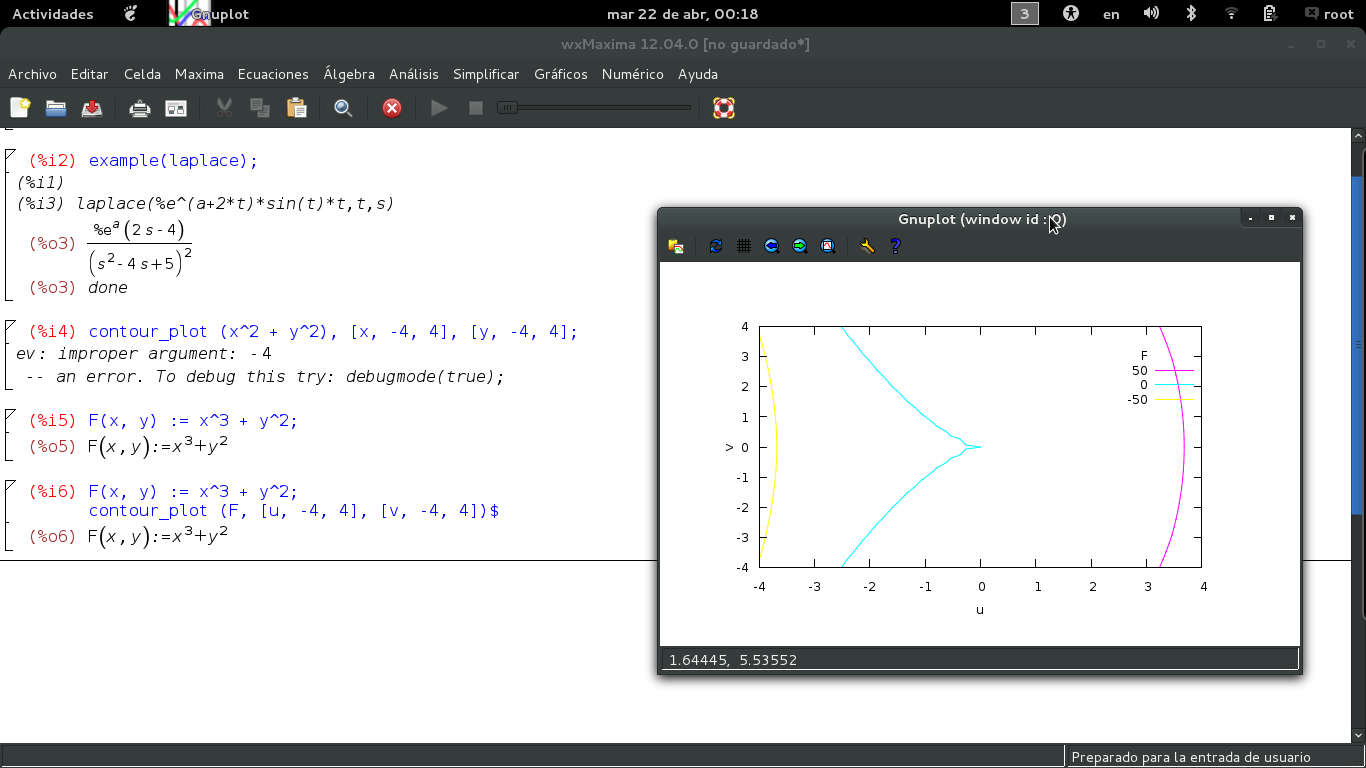
\includegraphics[width=13cm]{fotos/cap13}
\caption{\textbf{Ejemplo de graficacion}}
\end{center}
\end{figure}
\end{small}
\chapter{Comandos de wxMáxima}
\section{Editar}
Deshacer Control + z \\
Rehacer Control + Máyus + z \\
Cortar Control + X \\
Copiar Control + C \\
Copiar como Texto Máyus + Control + C \\
Pegar Control + V\\
Seleccionar todo Control + A
Buscar Control + F\\
Ampliar Alt + I\\
Disminuir Alt + O\\
\section{Celdas}
Evaluar Celda Máyus + Enter \\
Evaluar todas las celdas visibles Control + R\\
Evaluar todas las celdas Mayús+Control +R\\
Copiar entrada Anterior Control + I\\
Copiar salida anterior Control + U\\
Autocompletar Control + K\\
Mostrar Plantilla Mayús + Control + K\\
Nueva celda de texto Control + 1\\
Nueva celda de título Control + 2\\
Nueva delda de sección Control + 3\\
Nueva celda de subsección Control +4\\
Recoger todas las celdas Control + Alt+[ \\
Desplegar todas las celdas Control + Alt + ] \\
Instrucción Anterior Alt + Arriba \\
Siguiente Instrucción Alt + Abajo \\

\chapter{Tipos de Datos y Estructuras de Máxima}
\section{Números} 
Máxima puede trabajar con varios tipos de números así con números enteros, números racionales y números complejos
Una operación basica que Máxima puede hacer es la suma de enteros:\\

\noindent
%%%%%%%%%%%%%%%
%%% INPUT:
\begin{minipage}[t]{8ex}{\color{red}\bf
\begin{verbatim}
(%i1) 
\end{verbatim}}
\end{minipage}
\begin{minipage}[t]{\textwidth}{\color{blue}
\begin{verbatim}
3+5;
\end{verbatim}}
\end{minipage}
%%% OUTPUT:
\definecolor{labelcolor}{RGB}{100,0,0}
\begin{math}\displaystyle
\parbox{8ex}{\color{labelcolor}(\%o1) }
8
\end{math}
%%%%%%%%%%%%%%%

Igualmente en el caso de los racionales podemos realizar una operación similar: \\

\noindent
%%%%%%%%%%%%%%%
%%% INPUT:
\begin{minipage}[t]{8ex}{\color{red}\bf
\begin{verbatim}
(%i2) 
\end{verbatim}}
\end{minipage}
\begin{minipage}[t]{\textwidth}{\color{blue}
\begin{verbatim}
1/3-3/5;
\end{verbatim}}
\end{minipage}
%%% OUTPUT:
\definecolor{labelcolor}{RGB}{100,0,0}
\begin{math}\displaystyle
\parbox{8ex}{\color{labelcolor}(\%o2) }
\frac{-4}{15}
\end{math}
%%%%%%%%%%%%%%%
Máxima tambien puede trabajar con números complejos ,es así que para representar la parte real se usa el operador \textbf{\%i}

\noindent
%%%%%%%%%%%%%%%
%%% INPUT:
\begin{minipage}[t]{8ex}{\color{red}\bf
\begin{verbatim}
(%i3) 
\end{verbatim}}
\end{minipage}
\begin{minipage}[t]{\textwidth}{\color{blue}
\begin{verbatim}
(2+3*%i)*(6+2*%i);
\end{verbatim}}
\end{minipage}
%%% OUTPUT:
\definecolor{labelcolor}{RGB}{100,0,0}
\begin{math}\displaystyle
\parbox{8ex}{\color{labelcolor}(\%o3) }
\left( 2\,i+6\right) \,\left( 3\,i+2\right) 
\end{math}
%%%%%%%%%%%%%%%

\section{Operaciones Básicas Con Números Complejos}
Con los números complejos se pueden hacer las siguientes operaciones: \\
\textbf{realpart: } Devuelve el valor real de un número complejo\\

\noindent
%%%%%%%%%%%%%%%
%%% INPUT:
\begin{minipage}[t]{8ex}{\color{red}\bf
\begin{verbatim}
(%i4) 
\end{verbatim}}
\end{minipage}
\begin{minipage}[t]{\textwidth}{\color{blue}
\begin{verbatim}
realpart(3+7*%i);
\end{verbatim}}
\end{minipage}
%%% OUTPUT:
\definecolor{labelcolor}{RGB}{100,0,0}
\begin{math}\displaystyle
\parbox{8ex}{\color{labelcolor}(\%o4) }
3
\end{math}
%%%%%%%%%%%%%%%
\\ \textbf{imagpart: } Devuelve el valor imaginario de un número complejo\\

\noindent
%%%%%%%%%%%%%%%
%%% INPUT:
\begin{minipage}[t]{8ex}{\color{red}\bf
\begin{verbatim}
(%i5) 
\end{verbatim}}
\end{minipage}
\begin{minipage}[t]{\textwidth}{\color{blue}
\begin{verbatim}
imagpart(3+7*%i);
\end{verbatim}}
\end{minipage}
%%% OUTPUT:
\definecolor{labelcolor}{RGB}{100,0,0}
\begin{math}\displaystyle
\parbox{8ex}{\color{labelcolor}(\%o5) }
7
\end{math}
%%%%%%%%%%%%%%%
\\ \textbf{rectform: } Devuelve la fórmula rectangular de un número complejo\\

\noindent
%%%%%%%%%%%%%%%
%%% INPUT:
\begin{minipage}[t]{8ex}{\color{red}\bf
\begin{verbatim}
(%i6) 
\end{verbatim}}
\end{minipage}
\begin{minipage}[t]{\textwidth}{\color{blue}
\begin{verbatim}
rectform(3+7*%i);
\end{verbatim}}
\end{minipage}
%%% OUTPUT:
\definecolor{labelcolor}{RGB}{100,0,0}
\begin{math}\displaystyle
\parbox{8ex}{\color{labelcolor}(\%o6) }
7\,i+3
\end{math}
%%%%%%%%%%%%%%%
\\ \textbf{polarform: } Devuelve la forma polar de un número complejo\\

\noindent
%%%%%%%%%%%%%%%
%%% INPUT:
\begin{minipage}[t]{8ex}{\color{red}\bf
\begin{verbatim}
(%i7) 
\end{verbatim}}
\end{minipage}
\begin{minipage}[t]{\textwidth}{\color{blue}
\begin{verbatim}
polarform(3+7*%i);
\end{verbatim}}
\end{minipage}
%%% OUTPUT:
\definecolor{labelcolor}{RGB}{100,0,0}
\begin{math}\displaystyle
\parbox{8ex}{\color{labelcolor}(\%o7) }
\sqrt{58}\,{e}^{i\,\mathrm{atan}\left( \frac{7}{3}\right) }
\end{math}
%%%%%%%%%%%%%%%
\\ \textbf{cabs: } Devuelve la norma de un número complejo

\noindent
%%%%%%%%%%%%%%%
%%% INPUT:
\begin{minipage}[t]{8ex}{\color{red}\bf
\begin{verbatim}
(%i8) 
\end{verbatim}}
\end{minipage}
\begin{minipage}[t]{\textwidth}{\color{blue}
\begin{verbatim}
cabs(3+7*%i);
\end{verbatim}}
\end{minipage}
%%% OUTPUT:
\definecolor{labelcolor}{RGB}{100,0,0}
\begin{math}\displaystyle
\parbox{8ex}{\color{labelcolor}(\%o8) }
\sqrt{58}
\end{math}
%%%%%%%%%%%%%%%
\\ \textbf{carg: } Devuelve el valor del argumento del número complejo \\

\noindent
%%%%%%%%%%%%%%%
%%% INPUT:
\begin{minipage}[t]{8ex}{\color{red}\bf
\begin{verbatim}
(%i9) 
\end{verbatim}}
\end{minipage}
\begin{minipage}[t]{\textwidth}{\color{blue}
\begin{verbatim}
carg(3+7*%i);
\end{verbatim}}
\end{minipage}
%%% OUTPUT:
\definecolor{labelcolor}{RGB}{100,0,0}
\begin{math}\displaystyle
\parbox{8ex}{\color{labelcolor}(\%o9) }
\mathrm{atan}\left( \frac{7}{3}\right) 
\end{math}
%%%%%%%%%%%%%%%
\\ \textbf{conjugate: } Devuelve el conjugado de un número complejo

\noindent
%%%%%%%%%%%%%%%
%%% INPUT:
\begin{minipage}[t]{8ex}{\color{red}\bf
\begin{verbatim}
(%i10) 
\end{verbatim}}
\end{minipage}
\begin{minipage}[t]{\textwidth}{\color{blue}
\begin{verbatim}
conjugate(3+7*%i);
\end{verbatim}}
\end{minipage}
%%% OUTPUT:
\definecolor{labelcolor}{RGB}{100,0,0}
\begin{math}\displaystyle
\parbox{8ex}{\color{labelcolor}(\%o10) }
3-7\,i
\end{math}
%%%%%%%%%%%%%%%
\\ \textbf{csign: } Devuelve el tipo de número ingresado

\noindent
%%%%%%%%%%%%%%%
%%% INPUT:
\begin{minipage}[t]{8ex}{\color{red}\bf
\begin{verbatim}
(%i11) 
\end{verbatim}}
\end{minipage}
\begin{minipage}[t]{\textwidth}{\color{blue}
\begin{verbatim}
csign(3+7*%i);
\end{verbatim}}
\end{minipage}
%%% OUTPUT:
\definecolor{labelcolor}{RGB}{100,0,0}
\begin{math}\displaystyle
\parbox{8ex}{\color{labelcolor}(\%o11) }
complex
\end{math}
%%%%%%%%%%%%%%%

\section{Sistema de Ecuaciones con números complejos}
Un sistema simultaneo de Ecuaciones puede ser resuelto por Máxima incluso si tiene números complejos,con el comando \textbf{linsolve([ecuacion1],[ecuacion2], [variables])} , ejemplo: \\

\noindent
%%%%%%%%%%%%%%%
%%% INPUT:
\begin{minipage}[t]{8ex}{\color{red}\bf
\begin{verbatim}
(%i13) 
\end{verbatim}}
\end{minipage}
\begin{minipage}[t]{\textwidth}{\color{blue}
\begin{verbatim}
linsolve([(1+%i)*x-%i*y=2, (2+%i)*x + (2-%i)*y=2*%i], [x,y]);
\end{verbatim}}
\end{minipage}
%%% OUTPUT:
\definecolor{labelcolor}{RGB}{100,0,0}
\begin{math}\displaystyle
\parbox{8ex}{\color{labelcolor}(\%o13) }
[x=-\frac{10\,i+2}{13},y=\frac{18\,i-12}{13}]
\end{math}
%%%%%%%%%%%%%%%

\section{Operaciones con Límites}
Máxima puede calcular los límites (también complejos) de funciones, con la función \textbf{limit} evalua un límite así un límite calculado en el punto $\%2i$ se calcula así: 

\noindent
%%%%%%%%%%%%%%%
%%% INPUT:
\begin{minipage}[t]{8ex}{\color{red}\bf
\begin{verbatim}
(%i12) 
\end{verbatim}}
\end{minipage}
\begin{minipage}[t]{\textwidth}{\color{blue}
\begin{verbatim}
limit((-2*%i)^x, x, %i);
\end{verbatim}}
\end{minipage}
%%% OUTPUT:
\definecolor{labelcolor}{RGB}{100,0,0}
\begin{math}\displaystyle
\parbox{8ex}{\color{labelcolor}(\%o12) }
{2}^{i}\,{\left( - i\right) }^{i}
\end{math}
%%%%%%%%%%%%%%%
\\ Máxima puede también evaluar límites infinitos como se muestra a continuación: \\

\noindent
%%%%%%%%%%%%%%%
%%% INPUT:
\begin{minipage}[t]{8ex}{\color{red}\bf
\begin{verbatim}
(%i13) 
\end{verbatim}}
\end{minipage}
\begin{minipage}[t]{\textwidth}{\color{blue}
\begin{verbatim}
limit((-2*%i)*x, x, inf);
\end{verbatim}}
\end{minipage}
%%% OUTPUT:
\definecolor{labelcolor}{RGB}{100,0,0}
\begin{math}\displaystyle
\parbox{8ex}{\color{labelcolor}(\%o13) }
infinity
\end{math}
%%%%%%%%%%%%%%%
\section{Diferenciación de Complejos}
Con el comando \textbf{diff} Máxima puede devolver la derivada de un número, su sintaxis es: \textbf{diff(función,variable,número de veces a derivar)}

\noindent
%%%%%%%%%%%%%%%
%%% INPUT:
\begin{minipage}[t]{8ex}{\color{red}\bf
\begin{verbatim}
(%i15) 
\end{verbatim}}
\end{minipage}
\begin{minipage}[t]{\textwidth}{\color{blue}
\begin{verbatim}
diff((%i + 1)*x^{1/2},x,1);
\end{verbatim}}
\end{minipage}
%%% OUTPUT:
\definecolor{labelcolor}{RGB}{100,0,0}
\begin{math}\displaystyle
\parbox{8ex}{\color{labelcolor}(\%o15) }
\left( i+1\right) \,{\frac{1}{2}}\,{x}^{{\frac{1}{2}}-1}
\end{math}
%%%%%%%%%%%%%%%
\section{Integración de Complejos}
Para integrar complejos en Máxima debemos usar el comando \textbf{integrate(función,variable)} que nos muestra una salida así: 

\noindent
%%%%%%%%%%%%%%%
%%% INPUT:
\begin{minipage}[t]{8ex}{\color{red}\bf
\begin{verbatim}
(%i18) 
\end{verbatim}}
\end{minipage}
\begin{minipage}[t]{\textwidth}{\color{blue}
\begin{verbatim}
integrate((%i+1)*{1/2}*x^({1/2}-1), x);
\end{verbatim}}
\end{minipage}
%%% OUTPUT:
\definecolor{labelcolor}{RGB}{100,0,0}
\begin{math}\displaystyle
Is {\frac{1}{2}}-1 equal to -1?no;
\end{math}

\begin{math}\displaystyle
\parbox{8ex}{\color{labelcolor}(\%o18) }
\left( i+1\right) \,{x}^{{\frac{1}{2}}}
\end{math}
%%%%%%%%%%%%%%%


\end{document}